\chapter{Technické parametry testeru} \label{tehcnical parameters}
\section{Dlouhodobá stabilita}
Pro zjištění dlouhodobé stability byl proveden téměř 9-hodinový test běhu zařízení. Kde
každých 500\,ms byl ovládací kartě zasílán příkaz 80\_IO\_CARD MEASURE VOLTAGE ALL.
Výsledky měření pro piny 1 až 8 byly ukládány do textového souboru a následně zpracovány v programu MATLAB.
Zapojení testeru bylo provedeno dle schématu \ref{fig: 10hourTestScheme}.

\begin{figure}[ht!]
    \centering
    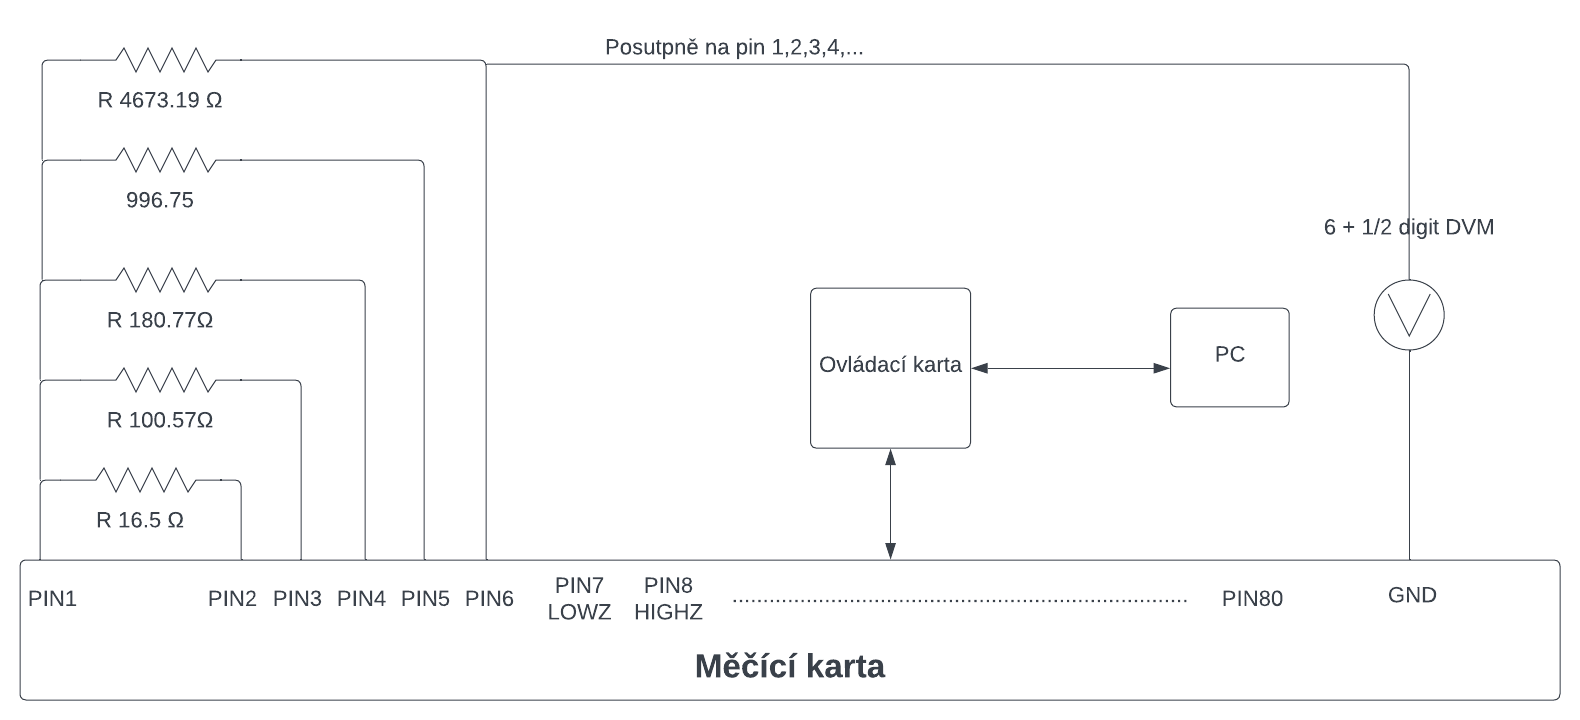
\includegraphics[width = 0.9\textwidth]{obrazky/10hourTestScheme.png}
    \caption{Dlouhodobá stabilita - schéma zapojení}
    \label{fig: 10hourTestScheme}
\end{figure}

Měřící karta byla nastavena do konfigurace na Obr. \ref{fig: 10hourTestConfig}. Tato konfigurace
umožňuje změřit propojení všech pinů do pinu č.1. Jedinou výjimkou je však nastavení pinu č. 8 do Vysoké impedance.

\begin{figure}[ht!]
    \centering
    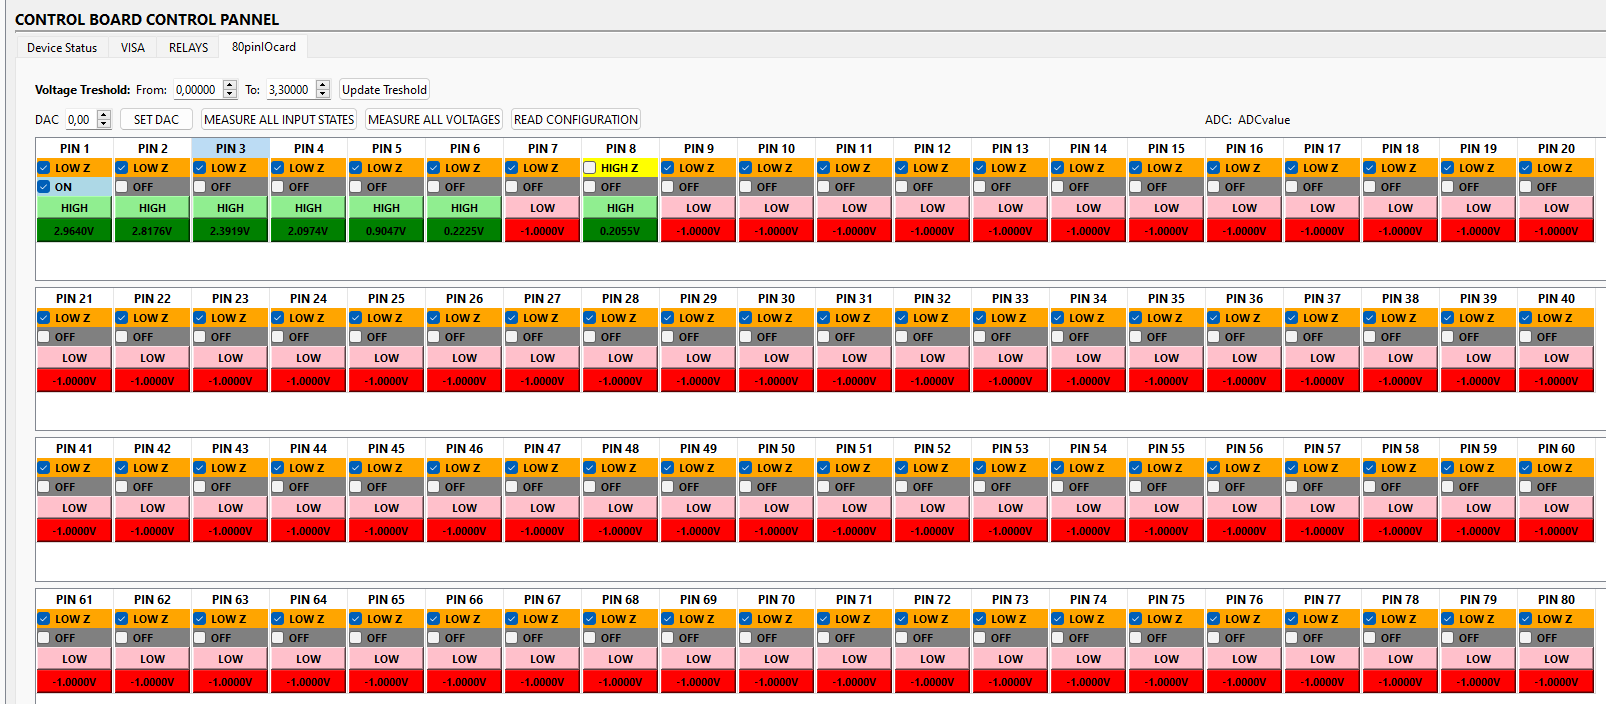
\includegraphics[width = 0.9\textwidth]{obrazky/10hourTestConfig.png}
    \caption{Dlouhodobá stabilita - Konfigurace měřící karty}
    \label{fig: 10hourTestConfig}
\end{figure}
\clearpage
Obrázek \ref{fig: 10hourTest ALL} zobrazuje průběhy napětí a všech zkoumaných pinech.
\begin{figure}[ht!]
    \centering
    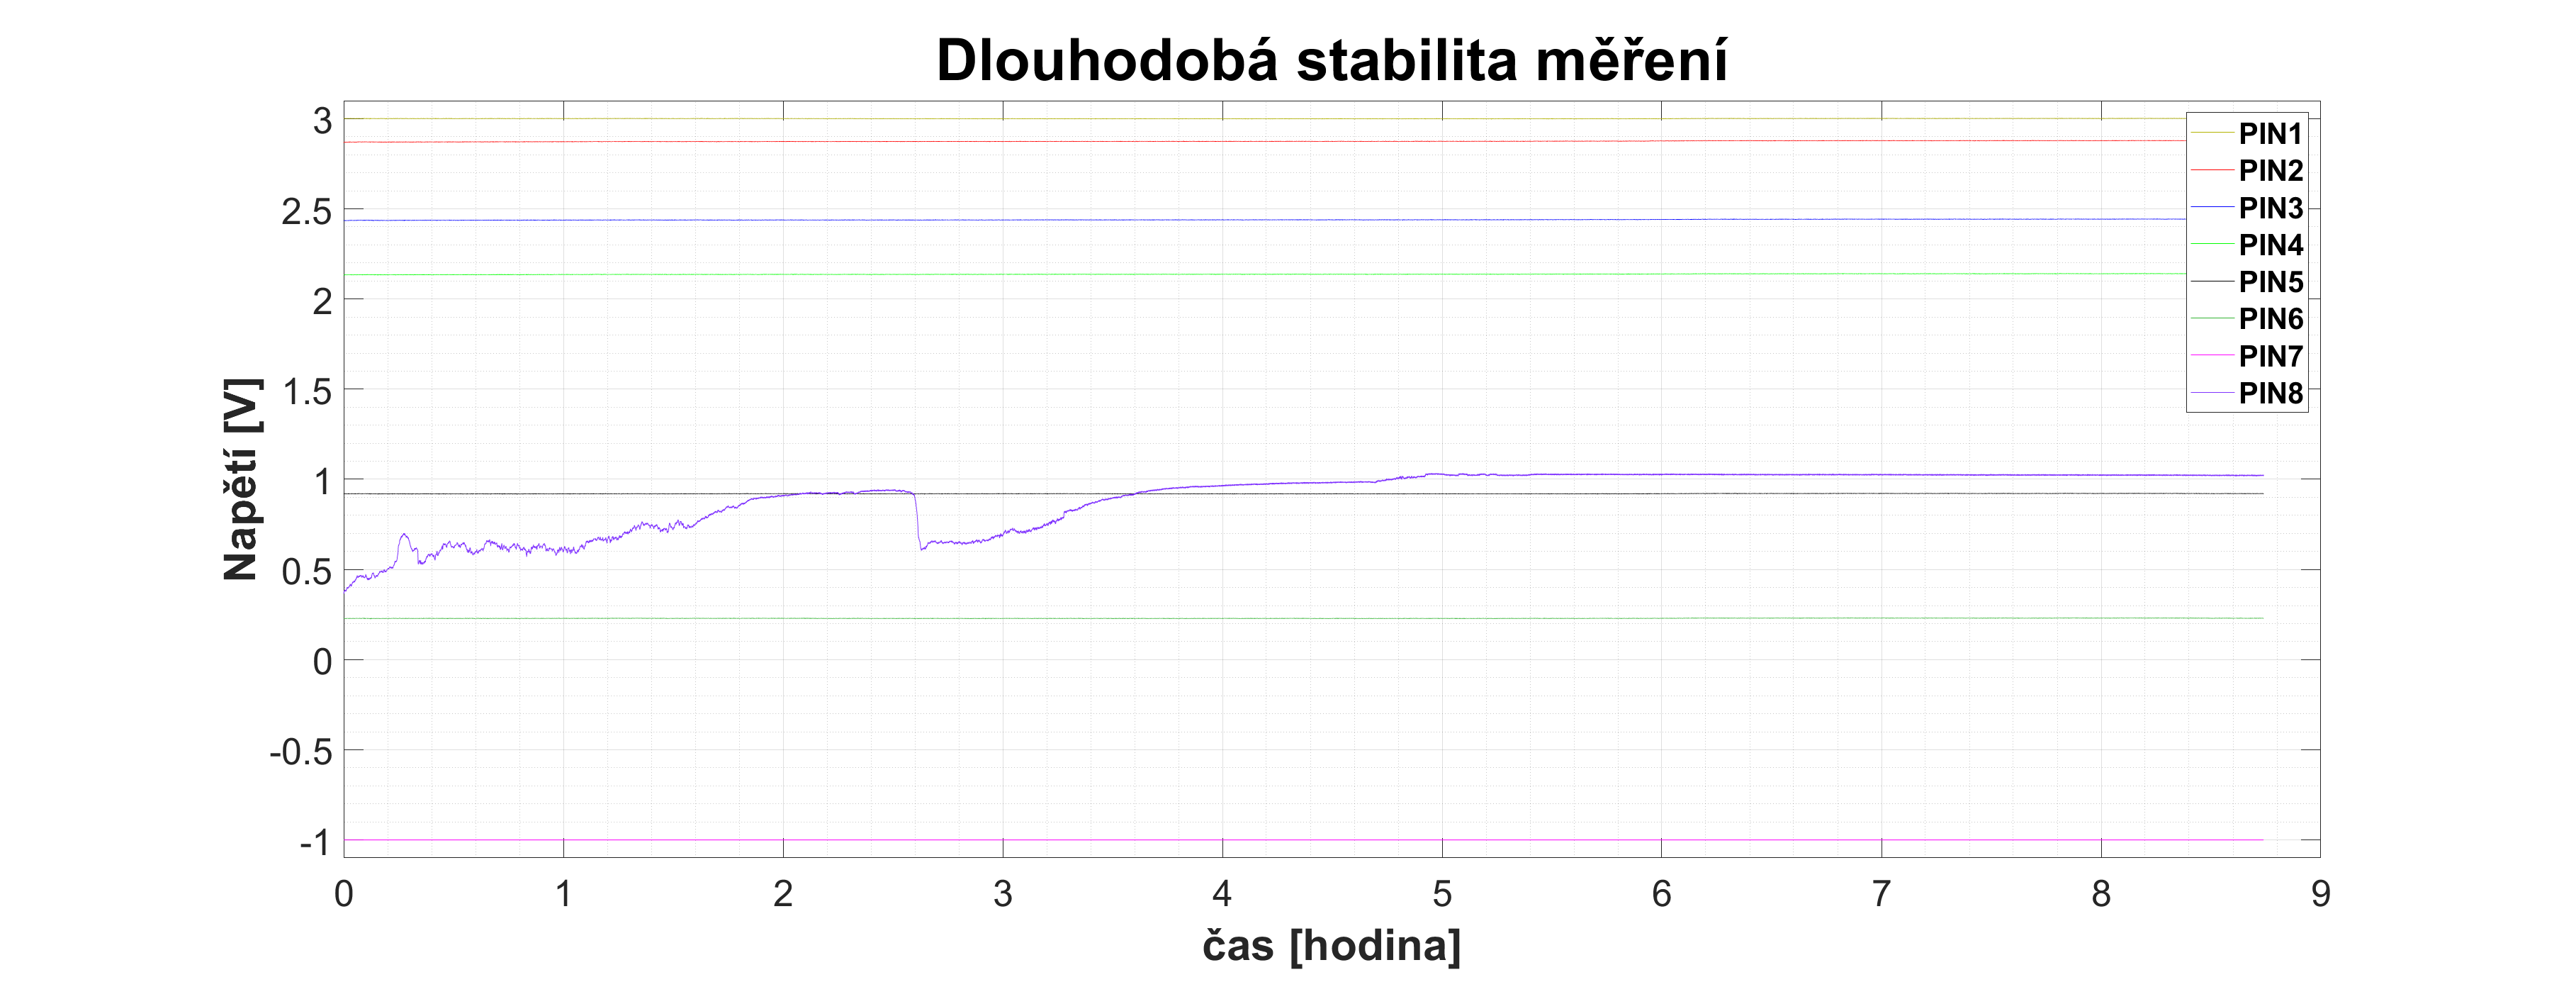
\includegraphics[width = 1\textwidth]{obrazky/matlab_generated/VOLTAGE_TESTER/dlouhodoba_stabilita_cas_prehled.eps}
    \caption{Dlouhodobá stabilita - Časový průběh všech naměřených napětí}
    \label{fig: 10hourTest ALL}
\end{figure}

Následující průběhy vycházejí z Obr. \ref{fig: 10hourTest ALL} a zobrazují detail časových průběhů napětí na jednotlivých pinech.
Podívejme se nejprve na průběh napětí na pinu č.7 (Obr. \ref{fig: 10hourTest Voltage PINS7TO8} nahoře).
Podle schématu (Obr. \ref{fig: 10hourTestScheme}) by pin č.7 neměl být nikam připojen a zároveň být v nízké impedanci. Očekává se tedy,
že měřené napětí bude velmi blízké nule. Ovládací karta vždy správně navrátila hodnotu -1,
která charakterizuje, že měřená hodnota je mimo rozsah měřící karty. Předpokládá se tak, že napětí je menší jak 70mV.\\

Pin č.8 je podle schématu zapojení (Obr. \ref{fig: 10hourTestScheme}) ve vysoké impedanci a zároveň není nikam připojen.
Impedance tohoto pinu je velmi vysoká (řádově stovky\,M$\Omega$) a pin chová nedefinovaně a může mít vesměs libovolnou hodnotu.
Během měření však změřená hodnota nepřekročila hodnotu přibližně 1.3V (Obr. \ref{fig: 10hourTest Voltage PINS7TO8} dole).
\begin{figure}[ht!]
    \centering
    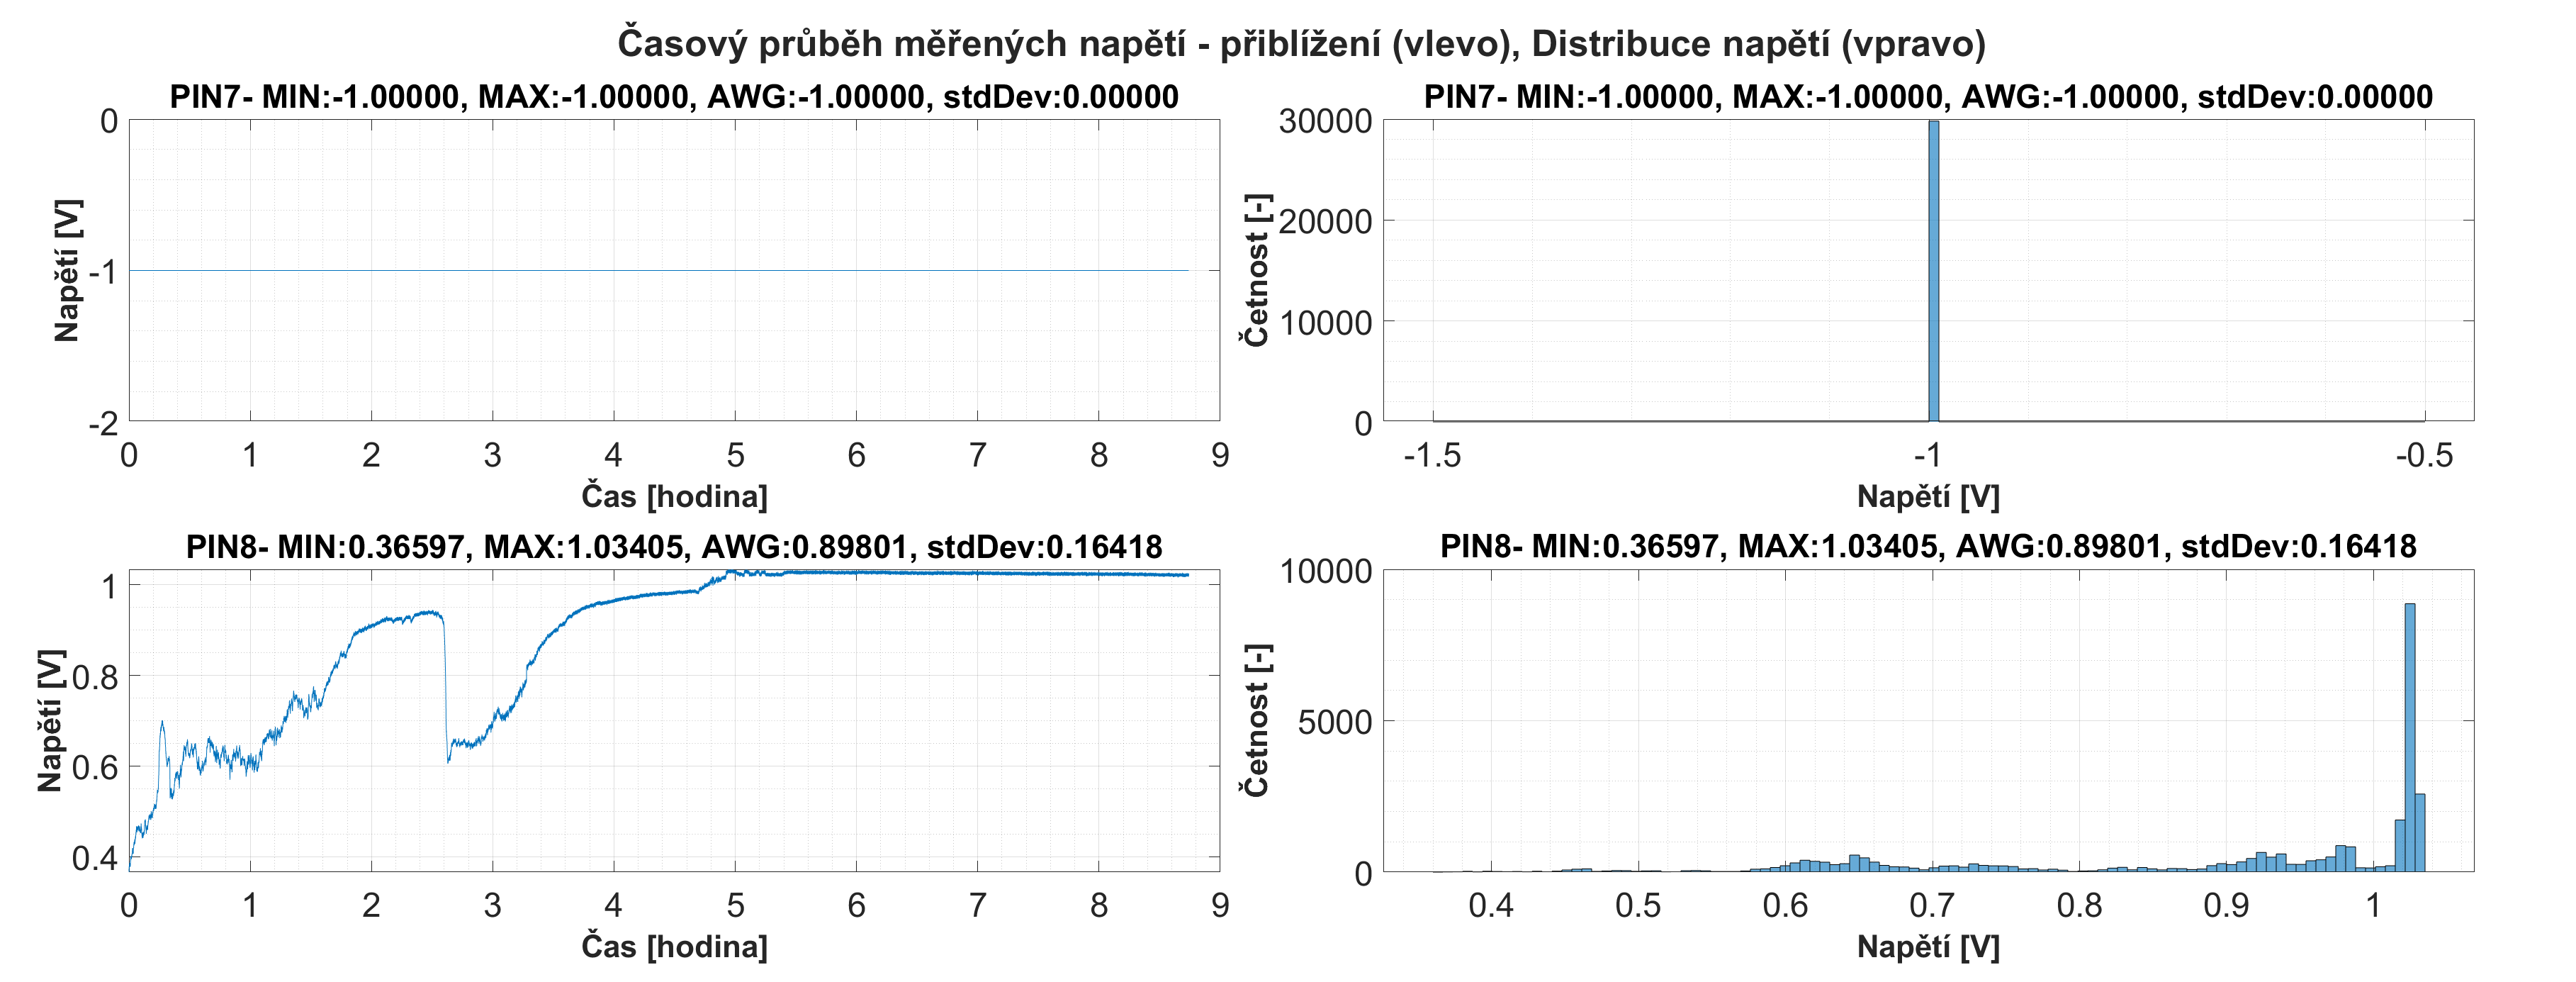
\includegraphics[width = 1\textwidth]{obrazky/matlab_generated/VOLTAGE_TESTER/dlouhodoba_stabilita_voltage_part2.eps}
    \caption{Dlouhodobá stabilita - Přiblížení časových průběhů napětí na pinech 7 až 8}
    \label{fig: 10hourTest Voltage PINS7TO8}
\end{figure}

\clearpage
Na následujícím obrázku jsou zobrazeny průběhy napětí na pinech 1 až 6.
V titulku každého grafu jsou uvedeny hodnoty průměru (AWG), MIN, MAX a směrodatné odchylky (stdDev) ve voltech.
Z histogramů je patrné, že rozptyl naměřených hodnot je větší než krok D/A převodníku o 1 bit
(každý ze sloupců je reprezentací určité bitové hodnoty). Lze tak v praxi uvažovat o nastavení kroku rampy
D/A převodníku na 2 bity . Tímto lze dosáhnout přibližně dvojnásobné rychlosti měření, přičemž se chyba měření příliš nezvýší.\\

\begin{figure}[ht!]
    \centering
    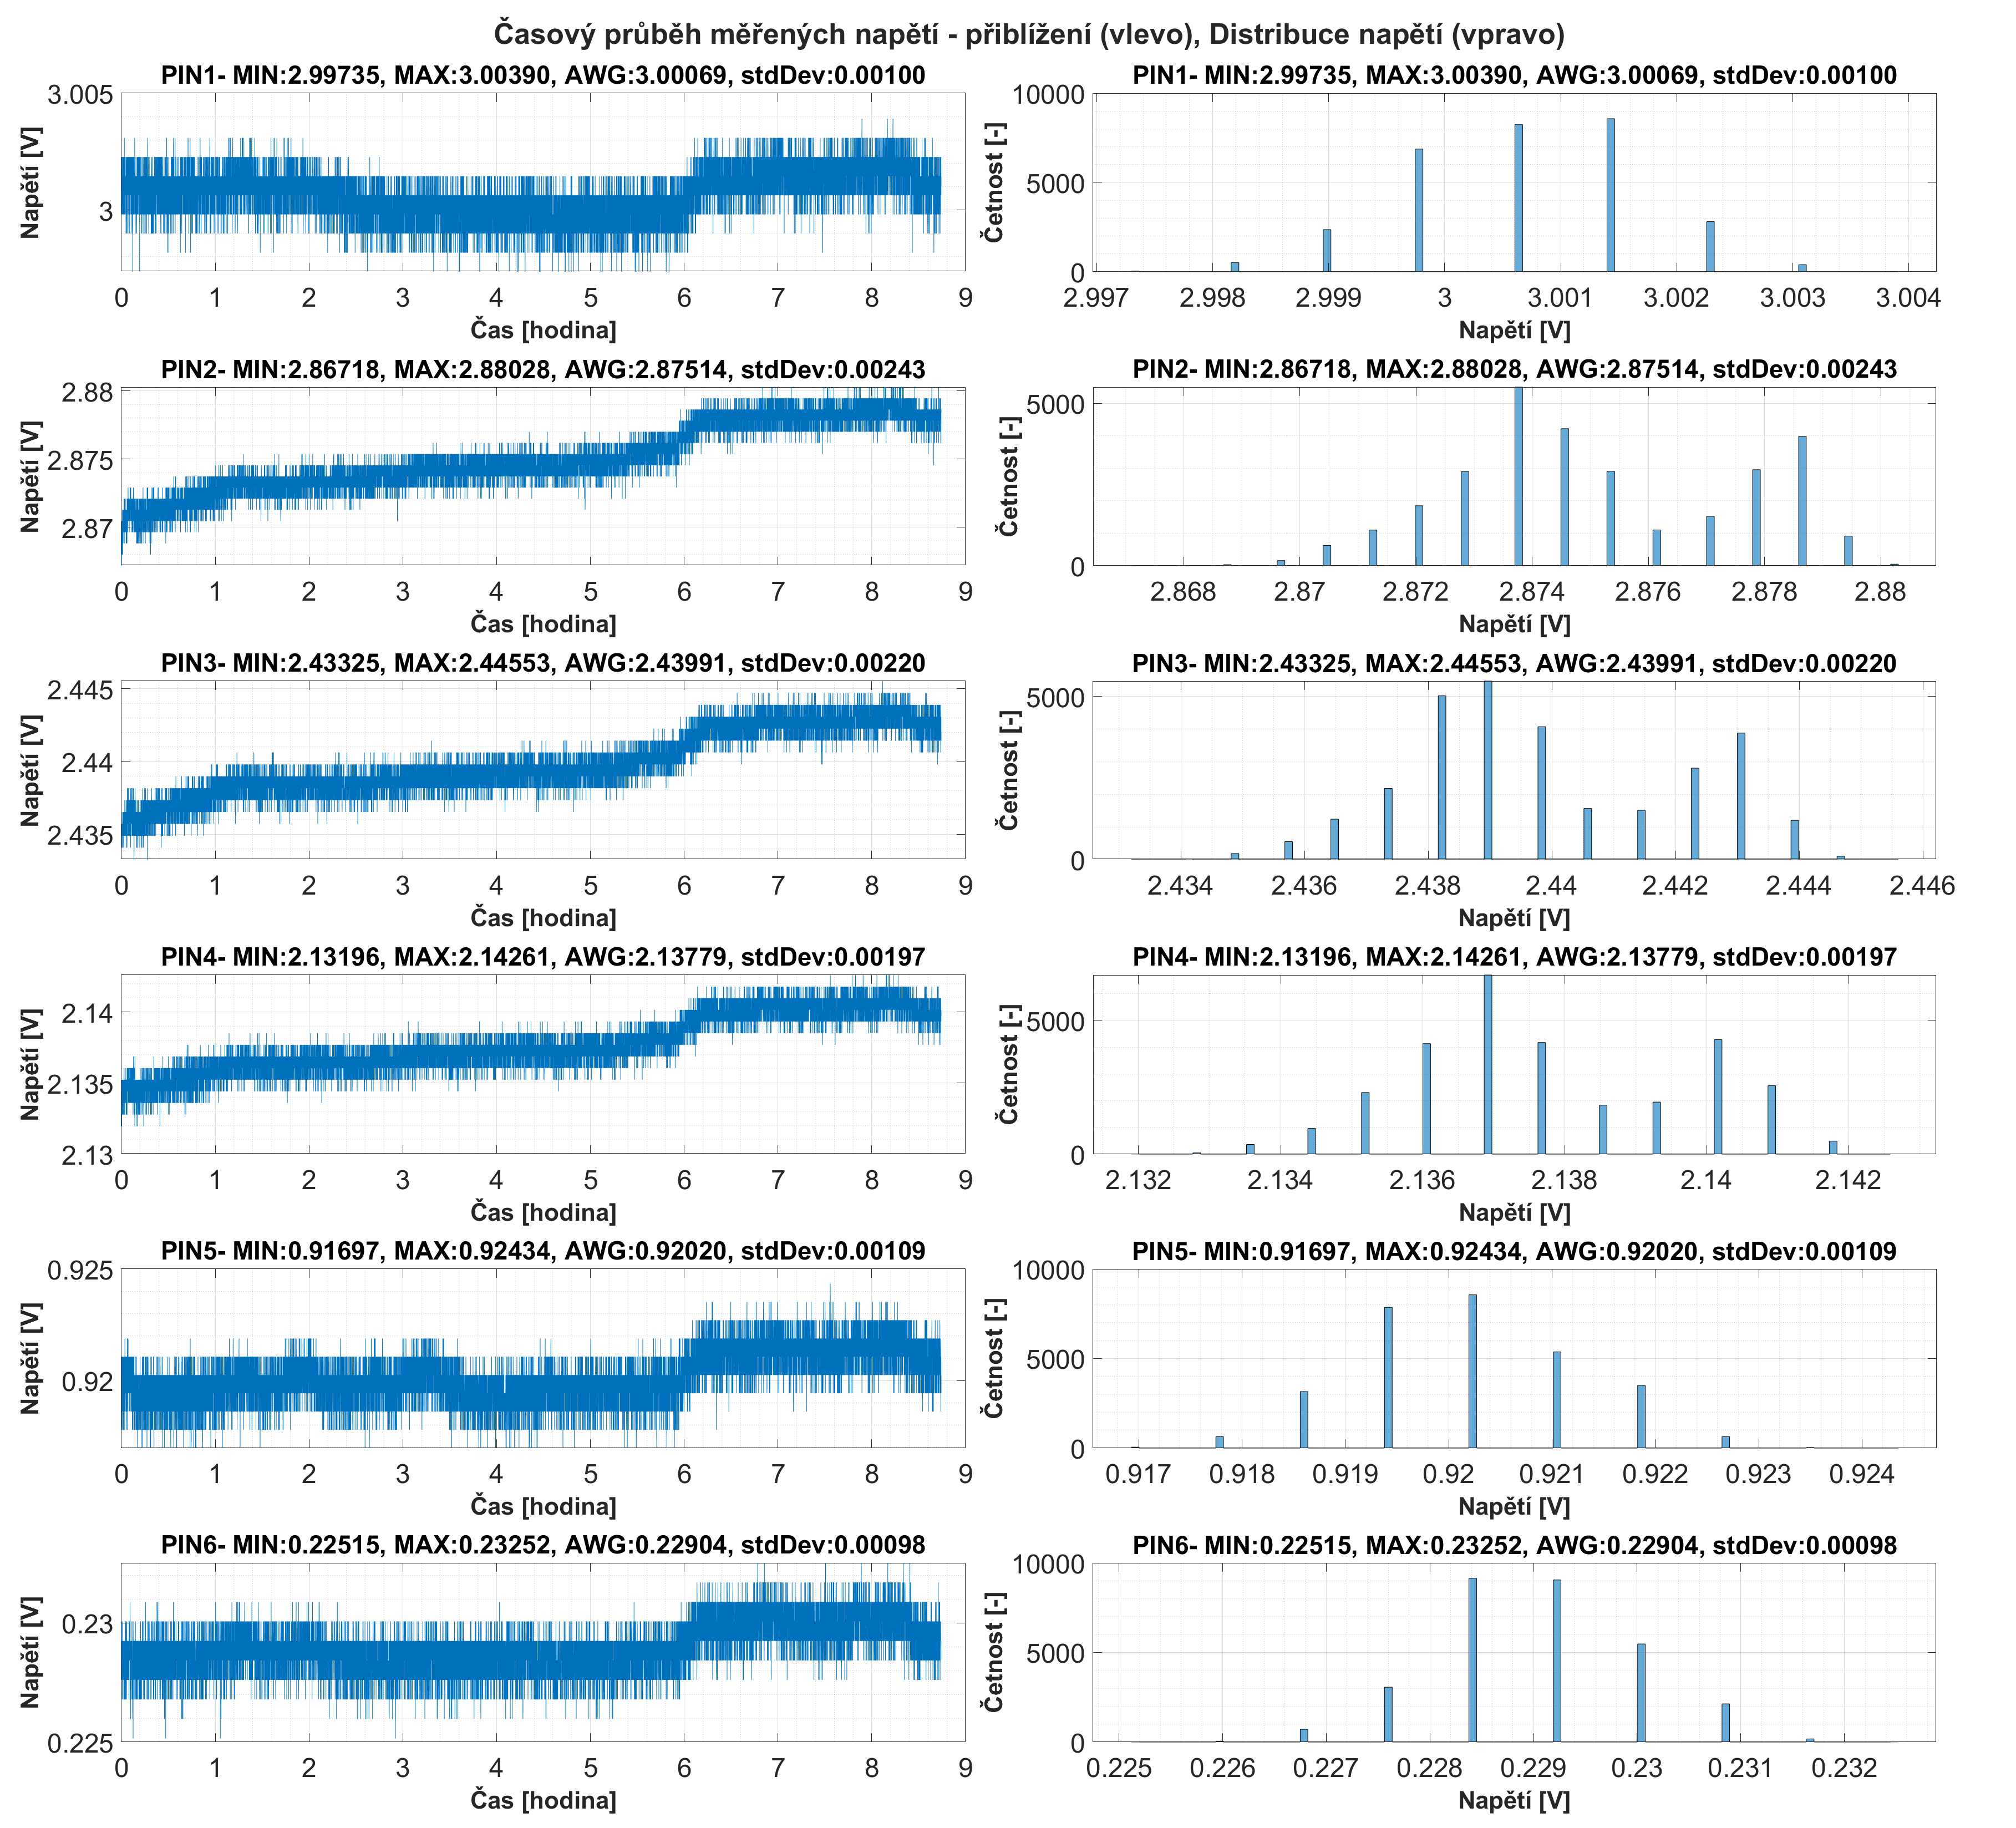
\includegraphics[width = 1\textwidth]{obrazky/matlab_generated/VOLTAGE_TESTER/dlouhodoba_stabilita_voltage_part1.eps}
    \caption{Dlouhodobá stabilita - Přiblížení časových průběhů napětí na pinech 1 až 6}
    \label{fig: 10hourTest Voltage PINS1TO4}
\end{figure}

Hlavním úkolem měření je však zjistit hodnoty odporů. Na Obr. \ref{fig: 10hourTest Resistor PINS1TO4}
jsou jednotlivé hodnoty z Obr({fig: 10hourTest Voltage PINS1TO4}) přepočítány na odpory vzhledem k pinu č.1.
Pro piny č.7 a 8 nemá příliš velký význam grafy uvádět, protože tyto piny nejsou nikam připojeny. Pin č.1 je připojen sám k sobě
a tak jeho hodnota odporu je nulová. V titulcích grafů lze obdobně jako u měřeného napětí nalézt statistické hodnoty a 
v titulcích u časových průběhů jsou zobrazeny i reálné hodnoty měřených odporů, které byly změřeny pomocí multimetru
GWINSTEK GDM-9061.\\

\clearpage
\begin{figure}[ht!]
    \centering
    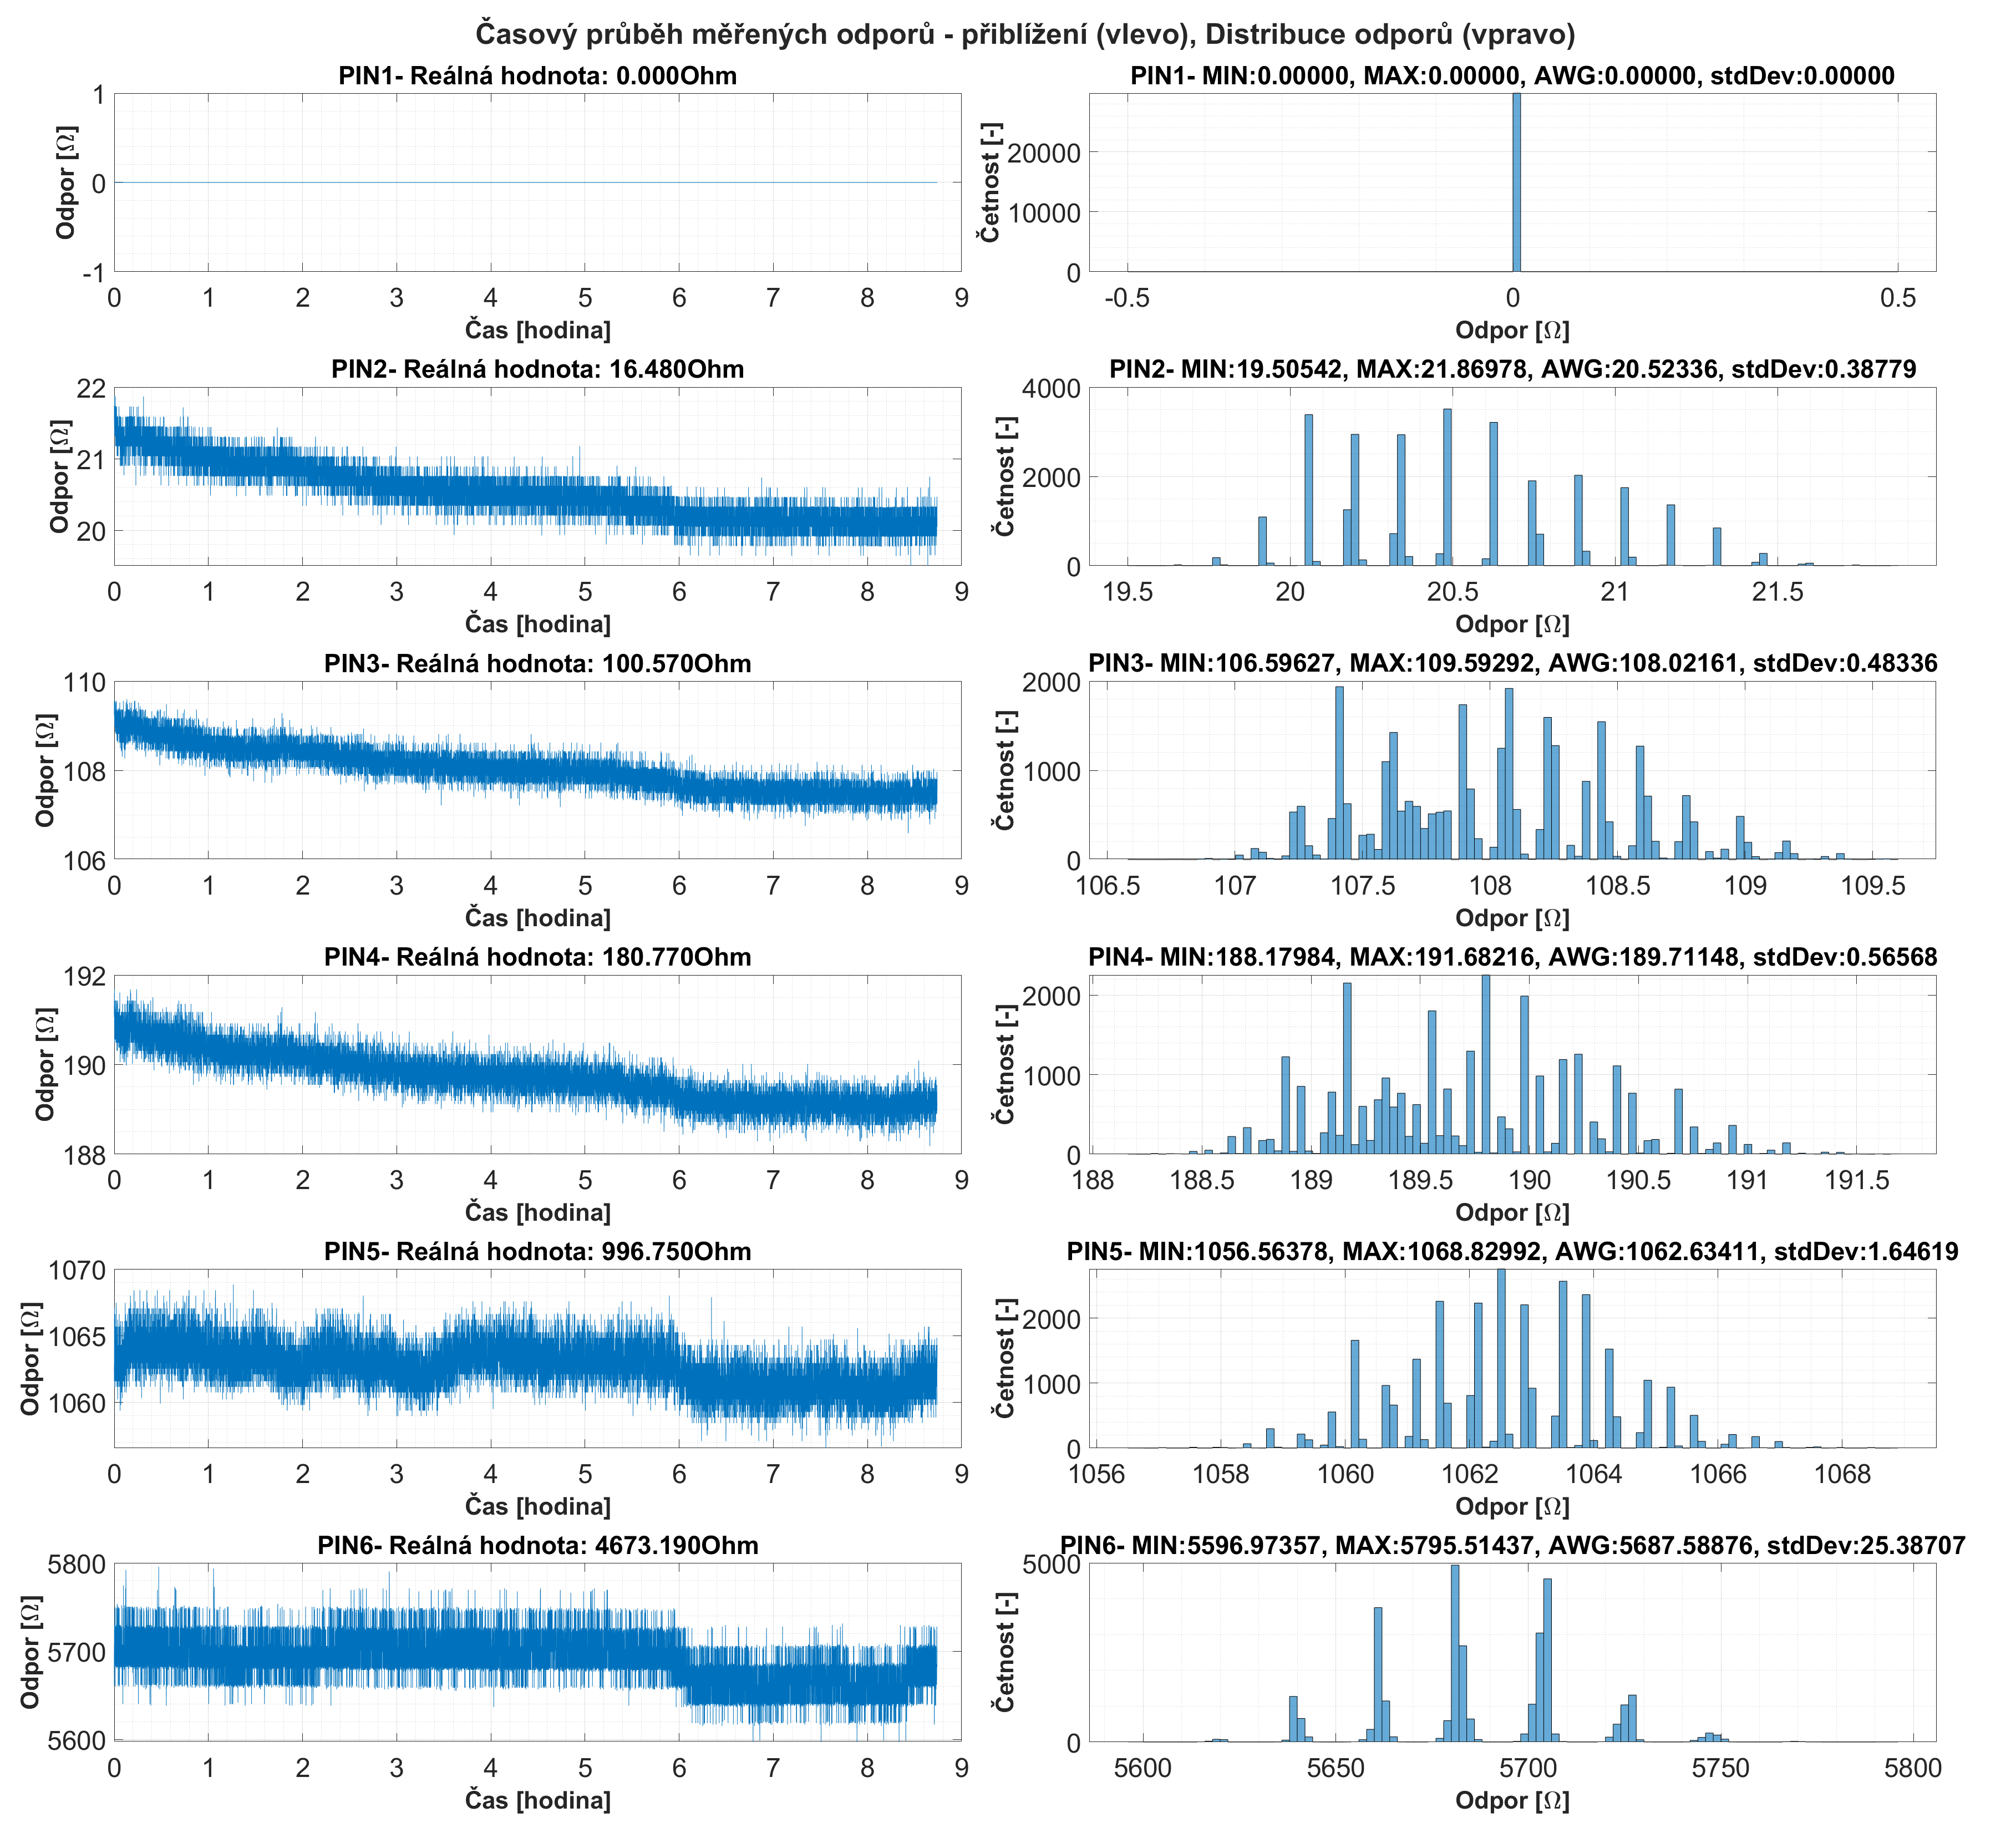
\includegraphics[width = 1\textwidth]{obrazky/matlab_generated/VOLTAGE_TESTER/dlouhodoba_stabilita_resistor_part1.eps}
    \caption{Dlouhodobá stabilita - Přiblížení časových průběhů odporů na pinech 1 až 6}
    \label{fig: 10hourTest Resistor PINS1TO4}
\end{figure}

Při porovnání změřených hodnot s reálnými je patrná odchylka v hodnotách odporů. Následující tabulka zobrazuje relativní a absolutní
chyby měření odporů vztaženou k průměrným naměřeným hodnotám. Tyto chyby jsou poměrně vysoké. Z tohoto důvodu je nutné měřící (respektive ovládací) karty kalibrovat.

\begin{table}[ht!]
    \centering
    \resizebox{0.7\textwidth}{!}{%
    \begin{tabular}{|l|l|l|l|l|l|}
    \hline
    \textbf{Chyba}          & \textbf{PIN2} & \textbf{PIN3} & \textbf{PIN4} & \textbf{PIN5} & \textbf{PIN6} \\ \hline
    \textbf{abs {[}$\Omega${]}}  & 4.043859      & 7.451614      & 8.941479      & 65.88411      & 1014.399      \\ \hline
    \textbf{rel {[}\%{]}} & 24.53872      & 7.40938       & 4.946329      & 6.609893      & 21.70677      \\ \hline
    \end{tabular}%
    }
    \caption{Chyby měření odporů vůči pinu č. 1 nezkalibrované měřící karty}
    \label{tab:chyby mereni necal}
    \end{table}

\clearpage
\section{Kalibrace}
Z důvodů zmíněných v předchozí sekci je nutné provádět kalibraci zařízení. Největší chyba měření je způsobena
chybou D/A převodníku. Tato chyba vzniká především kvůli saturacím při nejvyšších a nejnižších hodnotách napětí
v kombinaci se špatným nastavením referenčního napětí. Referenční napětí v předchozí sekci bylo nastaveno
následujícím způsobem.\\
Nejprve byla na D/A převodníku nastavena nejvyšší možná úroveň a poté bylo změřeno napětí na výstupu D/A převodníku
referenčním multimetrem. Obdržená hodnota napětí byla zapsána do ovládací karty a následně provedeno měření.
Všechny obdržené hodnoty napětí v tomto měření tak byly vztaženy k referenční hodnotě. Protože je však D/A převodník
ve své maximální hodnotě již saturován je vzniká pak chyba v interpretaci hodnot. Na obr. \ref{fig: 10hourTest calib DAC}
je modře znázorněna hodnota odvozená od referenčního napětí a červeně reálná hodnota napětí, kterou D/A převodník generuje.\\

\begin{figure}[ht!]
    \centering
    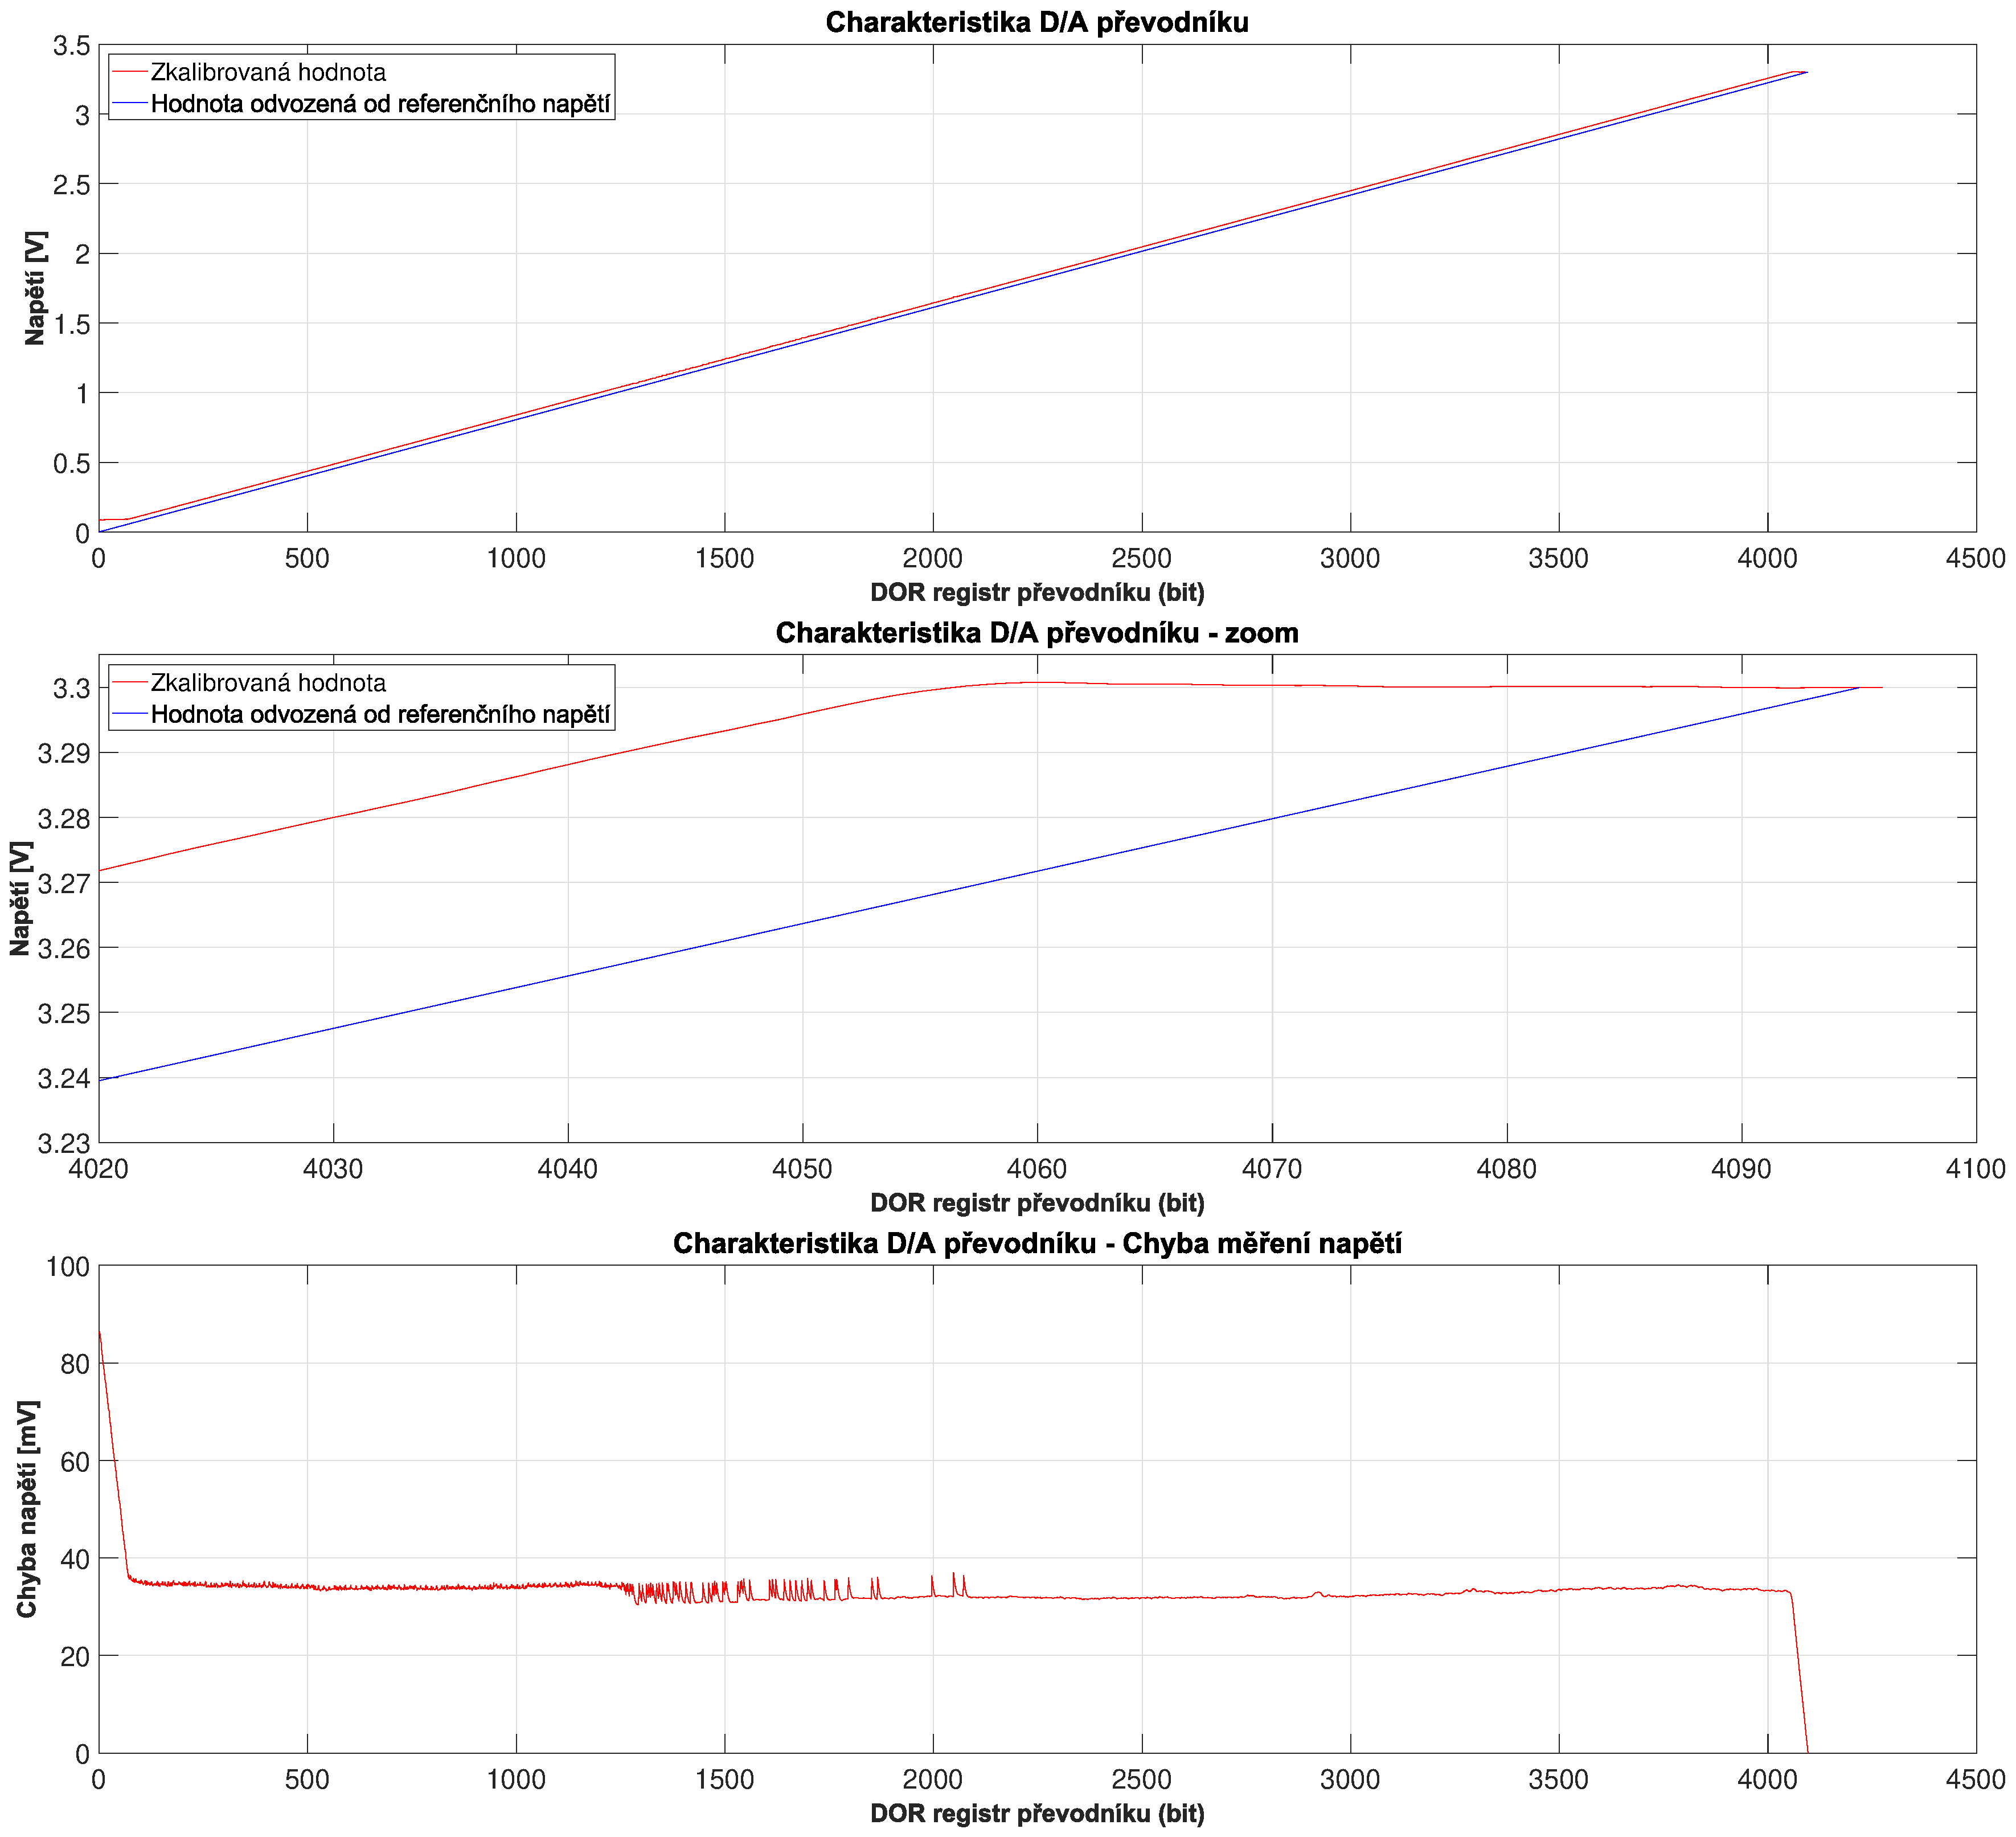
\includegraphics[width = 0.9\textwidth]{obrazky/matlab_generated/VOLTAGE_TESTER/calib_DAC.eps}
    \caption{Kalibrace D/A převodníku}
    \label{fig: 10hourTest calib DAC}
\end{figure}

Řešením tohoto problému je nejprve změřit výstupní hodnoty D/A převodníku pro každý jeho krok.
Toto měření je automatizováno a prováděno tak, že na výstup D/A převodníku je připojen referenční multimetr
a následně se pomocí kalibračního python skriptu uloží do mySQL databáze změřená hodnota pro každý krok D/A převodníku.\\

PC aplikace pak při měření nejprve nastaví referenční hodnotu napětí na 0xFFF (4095) čímž jsou obdržené hodnoty z ovládací karty
přímo nastavenými hodnotami registru D/A převodníku. PC aplikace následně využívá mySQL databázi jako lookup tabulku pro 
interpretaci přijatých hodnot. \\

Kalibrační hodnoty tak nejsou ukládány přímo do ovládací karty, ale do mySQL databáze. Takto lze poměrně snadno provádět kalibraci zpětně
již na změřená data. Na následujícím obrázku je jsou zobrazeny výsledky nového měření odporů po kalibraci.
Podmínky měření jsou stejné jako pro měření v předchozí sekci s rozdílem, že toto měření trvalo necelou hodinu.

\begin{figure}[ht!]
    \centering
    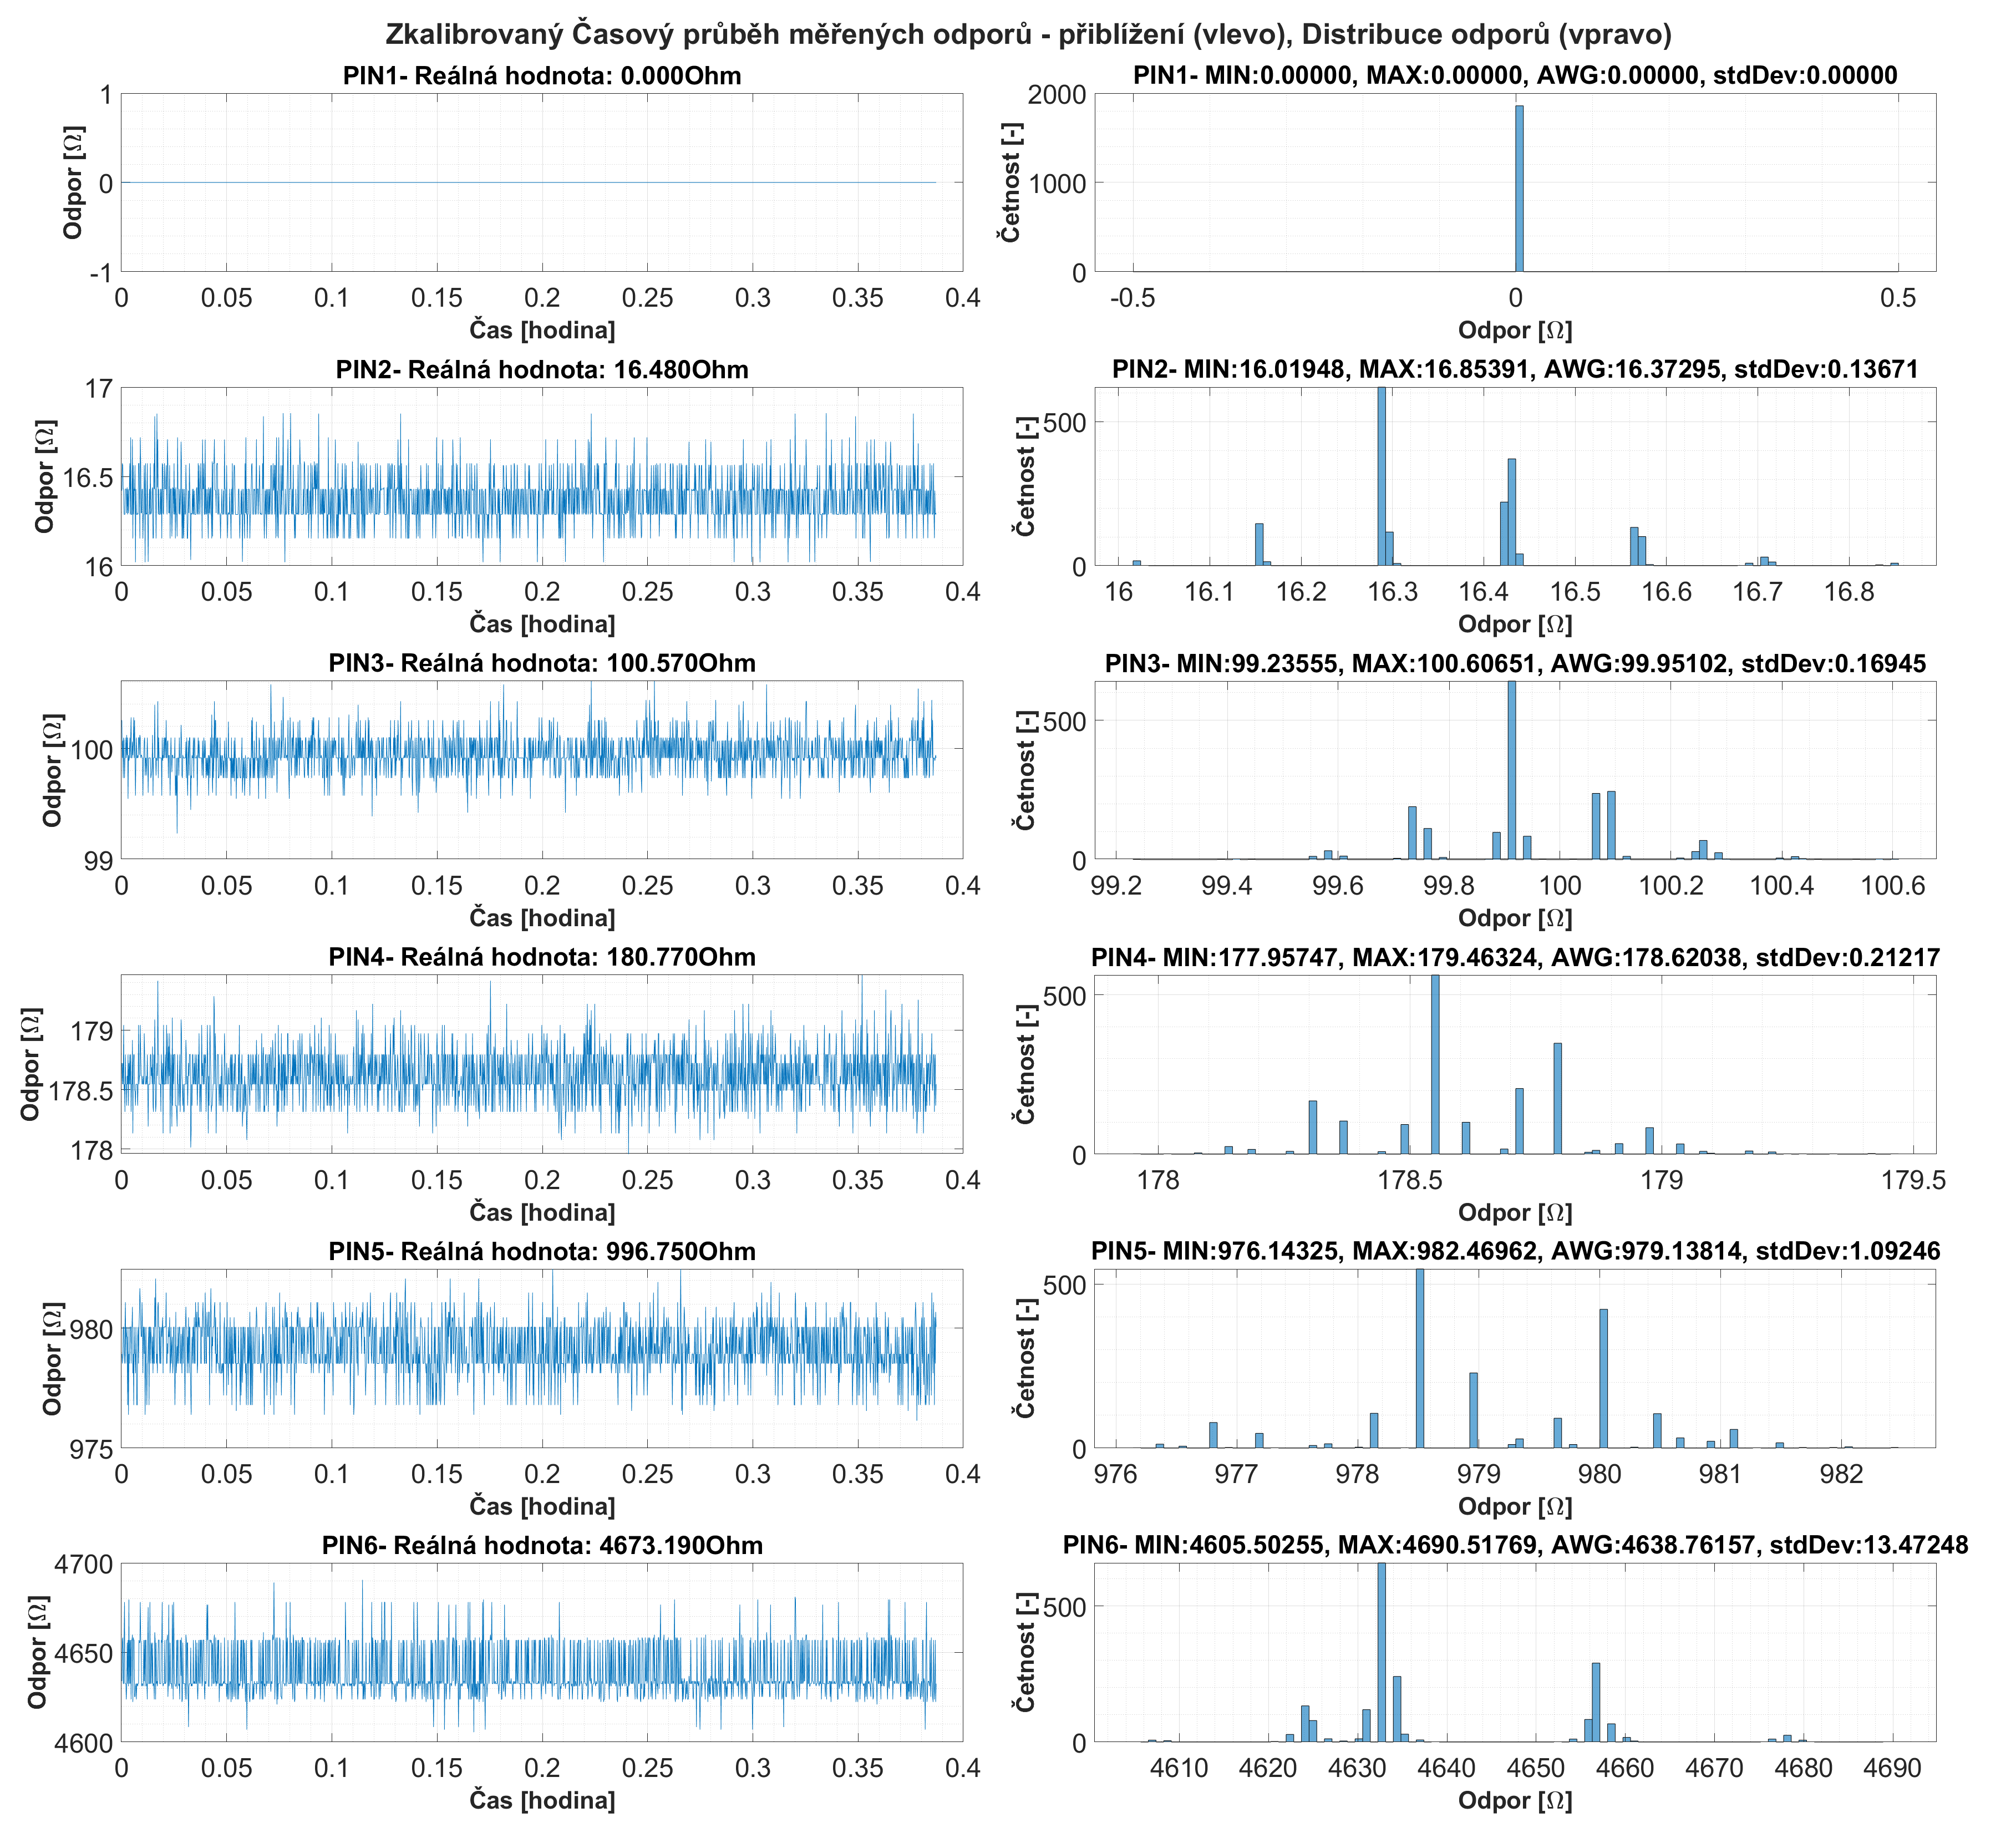
\includegraphics[width = 1\textwidth]{obrazky/matlab_generated/VOLTAGE_TESTER/calib_resistor_part1.eps}
    \caption{Dlouhodobá stabilita - Po kalibraci}
    \label{fig: 10hourTest calib Resistor PINS1TO6}
\end{figure}


    \clearpage
    V následující tabulce (\ref{tab:chyby mereni calibrated}) jsou zobrazeny hodnoty relativních a absolutních chyb měření
    vztažených k průměrné hodnotě naměřených hodnot po kalibraci.

    \begin{table}[ht!]
        \centering
        \resizebox{0.7\textwidth}{!}{%
        \begin{tabular}{|l|l|l|l|l|l|}
        \hline
        \textbf{Chyba}          & \textbf{PIN2} & \textbf{PIN3} & \textbf{PIN4} & \textbf{PIN5} & \textbf{PIN6} \\ \hline
        \textbf{abs {[}$\Omega${]}}  & 0.106549      & 0.618979      & 2.149619      & 17.61186      & 34.42843      \\ \hline
        \textbf{rel {[}\%{]}} & 0.646554      & 0.615471      & 1.189146      & 1.766929      & 0.736722      \\ \hline
        \end{tabular}%
        }
        \caption{Chyby měření po kalibraci odporů vůči pinu č. 1 nezkalibrované měřící karty}
        \label{tab:chyby mereni calibrated}
        \end{table}

    Z tabulky (\ref{tab:chyby mereni calibrated}) je patrné výrazné zlepšení chyb měření po kalibraci oproti nezkalibrovanému zařízení
    (tab.\ref{tab:chyby mereni necal}) .
    Dále by se dalo například zlepšit měření pomocí změření osazených rezistorů v napěťovém děliči pro každý bRC pin
    a následné korekce výpočtu odporu cesty. Nicméně vzhledem k dostatečné přesnosti
    měření a časové náročnosti dalších kalibračních procedur je proces kalibrace omezen pouze na kalibraci D/A převodníku.\\
